%%%%%%%%%%%%%%%%%%%%%%%%%%%%%%%%%%%%%%%%%%%%%%%%%%%%%%%%%%%%%%%%%%%%%%%%%%
%%  CHAPTER 1 -- INFERRING FIRMS' EMISSIONS FROM TRANSACTIONS DATA
%%  ~10 minutes. Frames lifted/trimmed from the inferring_emissions deck.
%%%%%%%%%%%%%%%%%%%%%%%%%%%%%%%%%%%%%%%%%%%%%%%%%%%%%%%%%%%%%%%%%%%%%%%%%%

%%%%%%%%%%%%%%%%%%%%% TEMPLATE-STYLE OVERVIEW %%%%%%%%%%%%%%%%%%%%%%%%%%%%
\begin{frame}{Inferring emissions: the problem in one slide}

    \begin{tcolorbox}[colback=green!5,colframe=green!40!black]
        \textbf{Question:} for the \emph{universe} of firms --- where emissions are
        unobserved --- how far can \textbf{B2B transaction data} take us in inferring
        firm-year emissions?
    \end{tcolorbox}

    \begin{wideitemize}
        \item[\alertg{Why hard:}] registries (EU ETS) \& surveys cover only \alertr{large installations}, in a handful of countries
        \pause
        \item[\alertb{Idea:}] firms that combust fossil fuels must \alerto{buy them} $\rightarrow$ purchases leave traces in the \alertp{transaction network}
        \pause
        \item[\alertoch{Data:}] Belgium --- near-universe B2B (2002--22) $+$ \alertg{verified EU ETS emissions} as ground truth
        \pause
        \item[\alertr{Result:}] a cross-fitted \alertp{elastic-net proxy} separates emitters from non-emitters (TPR 96\%, FPR $\le$17\%) and ranks them (Spearman $0.64$)
    \end{wideitemize}

\end{frame}

%%%%%%%%%%%%%%%%%%%%% TRAINING SAMPLE %%%%%%%%%%%%%%%%%%%%%%%%%%%%%%%%%%%%
\begin{frame}{Training sample: where the signal is learned}

    The set of firms we use to identify relevant suppliers:

    \begin{wideitemize}
        \item[\textbf{(i)}] \alertb{EU ETS firms}: 257 firms, 3,170 firm-years
        \begin{wideitemize}
            \item[-] verified yearly emissions from the EU Transaction Log
        \end{wideitemize}

        \item[\textbf{(ii)}] \alertg{Non-ETS firms in $\sim$100\%-covered sectors}: 2,959 firms, 23,438 firm-years
        \begin{wideitemize}
            \item[-] Petroleum refining (19), Iron \& steel (24), Paper, pulp \& print (17/18)
            \item[-] assigned \alerto{zero combustion emissions} (EU ETS covers $\sim$100\%)
        \end{wideitemize}
    \end{wideitemize}

    \vspace{0.3cm}
    \alertr{Why include the zeros?}
    $\rightarrow$ gives the model \alertb{extensive-margin} information;
    same sectors are \alerto{energy-intensive} $\Rightarrow$ a demanding test.

\end{frame}

%%%%%%%%%%%%%%%%%%%%% THE ELASTIC-NET APPROACH %%%%%%%%%%%%%%%%%%%%%%%%%%
\begin{frame}{Let the data identify the relevant suppliers}

    \begin{wideitemize}
        \item \alertb{Benchmark}: sum purchases from the six fuel-selling NACE codes
        \\ {\color{dgray}\small (Tabachova 2025, Stangl et al.\ 2026) --- misses multi-activity sellers, symmetric weights}

        \item \alertg{This paper}: regress verified emissions on \alertb{firm-year purchases from each supplier}
        $$ y_{it} = \sum_{j} \beta_j \, x_{ijt} + \gamma \log(\text{revenue}_{it}) + \boldsymbol{\delta}' \mathbf{d}_{t} + \boldsymbol{\phi}' \mathbf{s}_{i} + \varepsilon_{it} $$
        {\small $y_{it}=\operatorname{asinh}(\text{emissions})$, $x_{ijt}=\operatorname{asinh}(\text{sales})$; revenue \& FEs \alerto{unpenalized}}

        \item \alertp{Elastic-net penalty} on $\{\beta_j\}$ \;($\alpha=0.5$, $\lambda$ by firm-grouped CV)
        $\Rightarrow$ \alertb{EN-proxy}$_{it}=\!\!\sum_{j:|\hat\beta_j|>0}\!\!\hat\beta_j\,x_{ijt}$
    \end{wideitemize}

\end{frame}

%%%%%%%%%%%%%%%%%%%%% WHO ARE THE SELECTED SUPPLIERS %%%%%%%%%%%%%%%%%%%%
\begin{frame}{Who are the selected suppliers?}

    \begin{wideitemize}
        \item Out of $\sim$22,700 candidates, EN selects \alertb{612 suppliers} (463 $+$, 149 $-$)

        \item Dispersed across \alerto{53 NACE 2-digit sectors}:
        \begin{wideitemize}
            \item[-] largest: \alertp{wholesale trade (46)}; then construction, engineering, transport
            \item[-] \alertr{notably absent}: refined petroleum (19), electricity/gas (35)
        \end{wideitemize}

        \item Overlap with the NACE fuel-seller set is \alertr{minimal}: only \alertr{4 of 612} (0.7\%)

        \item[] \alertg{$\Rightarrow$ data-driven selection and NACE codes pick nearly disjoint sets of firms}
    \end{wideitemize}

\end{frame}

%%%%%%%%%%%%%%%%%%%%% EXTENSIVE-MARGIN VALIDATION %%%%%%%%%%%%%%%%%%%%%%%
\begin{frame}{The proxy separates emitters from non-emitters}

    \begin{columns}
    \begin{column}{0.6\textwidth}
        \begin{figure}
            \centering
            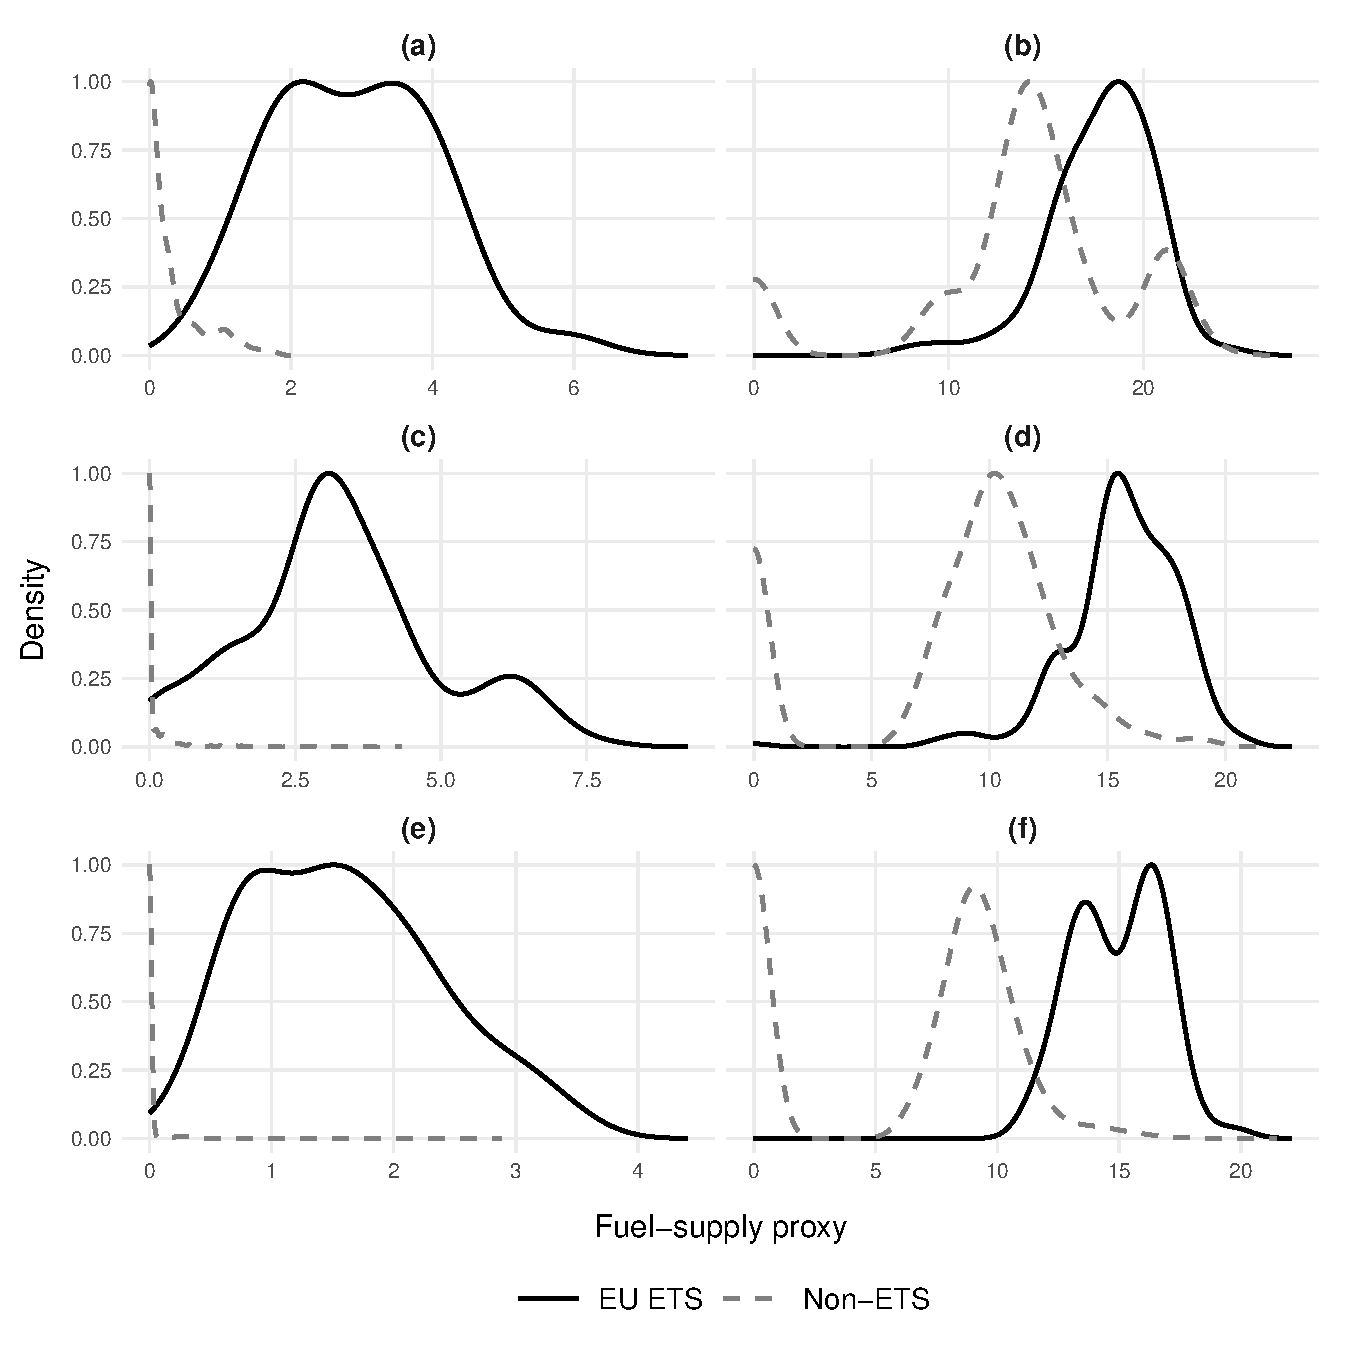
\includegraphics[width=\linewidth]{figures/proxy_density_by_emitter.pdf}
        \end{figure}
    \end{column}
    \begin{column}{0.4\textwidth}
        \begin{wideitemize}
            \item[] Kernel densities of the proxy
            \item[\alertb{Black}:] EU ETS firms
            \item[\alertr{Grey}:] non-ETS firms

            \item[]
            \item[] AUC (EN-proxy):
            \begin{wideitemize}
                \item[-] Petrol.\ ref.: \alertg{0.99}
                \item[-] Iron \& steel: \alertg{0.97}
                \item[-] Paper/print: \alertg{0.99}
            \end{wideitemize}
        \end{wideitemize}
    \end{column}
    \end{columns}

\end{frame}

%%%%%%%%%%%%%%%%%%%%% OUT-OF-SAMPLE RESULTS %%%%%%%%%%%%%%%%%%%%%%%%%%%%%
\begin{frame}{Out-of-sample performance (sector-level cross-fitting)}

    \begin{center}
    \scalebox{0.78}{
    \begin{tabular}{l ccc cc cccc}
    \toprule
     & \multicolumn{3}{c}{Prediction error} & \multicolumn{2}{c}{Correlation} & \multicolumn{4}{c}{Extensive margin} \\
    \cmidrule(lr){2-4} \cmidrule(lr){5-6} \cmidrule(lr){7-10}
     & RMSE & nRMSE & MAPD & Levels & Rank & FPR & TPR & p50 & p99 \\
    \midrule
    Revenue         & 190 & 1.00 & \alertg{0.71} & 0.85 & 0.53 & \alertr{1.00} & 1.00 & 0.01 & 0.39 \\
    Elastic Net     & 218 & 1.15 & 0.84 & 0.85 & \alertg{0.64} & \alertg{0.17} & 0.96 & 0.01 & \alertg{0.19} \\
    NACE            & 214 & 1.13 & 0.85 & 0.81 & 0.52 & 0.67 & 0.99 & 0.01 & 0.46 \\
    Gated Rev.\     & 193 & 1.01 & 0.71 & 0.84 & \alertg{0.68} & \alertg{0.17} & 0.96 & 0.00 & 0.35 \\
    Geom.\ Mean     & 218 & 1.15 & 0.74 & 0.83 & 0.63 & 0.26 & 0.97 & 0.01 & 0.28 \\
    \bottomrule
    \end{tabular}
    }
    \end{center}

    \begin{wideitemize}
        \item EN dominates the \alertg{extensive margin} (FPR $0.17$ vs.\ revenue $1.00$, NACE $0.67$)
        \item Revenue dominates \alertg{level accuracy among emitters} (MAPD $0.71$)
        \item \alerto{Gated Revenue} (EN classifies, revenue scales) $=$ best of both; rank corr.\ $0.68$
        \item[] {\footnotesize Means over $M=200$ sector-level CV repeats.}
    \end{wideitemize}

\end{frame}

%%%%%%%%%%%%%%%%%%%%% TAKEAWAYS %%%%%%%%%%%%%%%%%%%%%%%%%%%%%%%%%%%%%%%%%%
\begin{frame}{Chapter 1 --- takeaways}

    \begin{wideitemize}
        \item \alertb{B2B transaction data carry a signal about emissions} unavailable from balance-sheet variables alone

        \item A \alertp{cross-fitted elastic-net proxy} beats NACE classification, and a hybrid recovers the best of both margins

        \item \alertg{Broader lesson}: combustion $\Rightarrow$ fuel purchases $\Rightarrow$ network traces
        \begin{wideitemize}
            \item[-] a \alerto{general economic logic}, not Belgium-specific
            \item[-] testable wherever \alertp{transaction data $+$ a partial registry} coexist
        \end{wideitemize}

        \item[] {\color{dgray}\small $\hookrightarrow$ the same firm-level emissions \& network reappear, structurally, in Chapter~3.}
    \end{wideitemize}

\end{frame}
